	The interface for collecting survey data separates states such as simple, check, sink or terminate on different template views. The data validation is entirely performed in the client (e.g. checking that the number of chosen responses is between a range, ensuring that every row from a grid question contains at least one response selected or verifying data-types). These validations help to reduce the amount of operations to carry out between server and client. Additionally, as this interface reacts to events immediately, the user experience is greatly improved.

	The stateless restriction from our \gls{rest} architecture requires for each new interview carried out in a browser to persist the interviewee's identifier either by using cookies or through the browser's data storage. Similarly, when the questionnaire is completed, it is the responsibility of the client to delete this persisted id. Every time the navigation is updated, i.e. next or previous action is requested, the server responds with the new state reached and the client redraws the part of the interface that needs to be changed without the need for page reloading.
	
	Figure \ref{fig:impl:collectionInterface} represents an example of an interview demo that was presented at the \gls{xml} Prague conference 2015. %\cite{proc:lloret15}. 
	Firstly the display of the example question provides a language translation option in order to change to other languages. Next, it displays an example of a single question (e.g. Q1) with multiple responses represented through radio buttons. Finally, at the bottom, the navigation options (e.g. previous and next) are presented. Note that the next action appears disabled but it becomes enabled whenever the data entered for a question successfully passes the client validations.

	\begin{figure}[h]
	\centering
	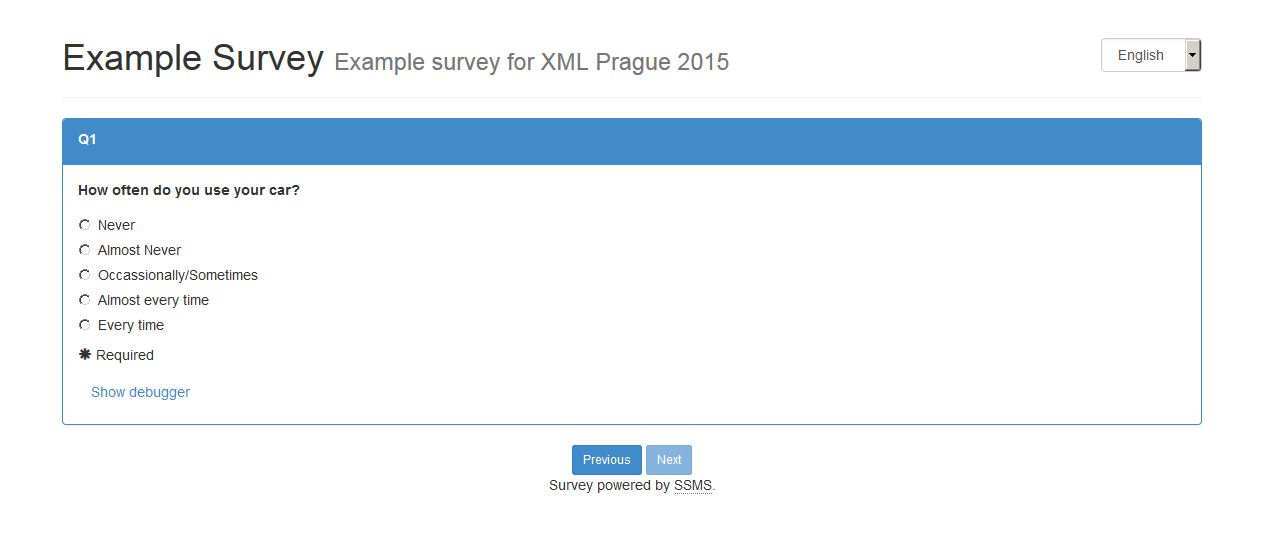
\includegraphics[width=0.90\textwidth]{implementation/img/collection}
	\caption{Collection interface}
	\label{fig:impl:collectionInterface}
	\end{figure}